% Generated 2020-10-22 16:25:25 +0530
\subsection{DataItems} \label{sec:DataItems}


\block{DataItems} \glspl{organize} \block{DataItem} elements.

\begin{figure}[ht]
  \centering
    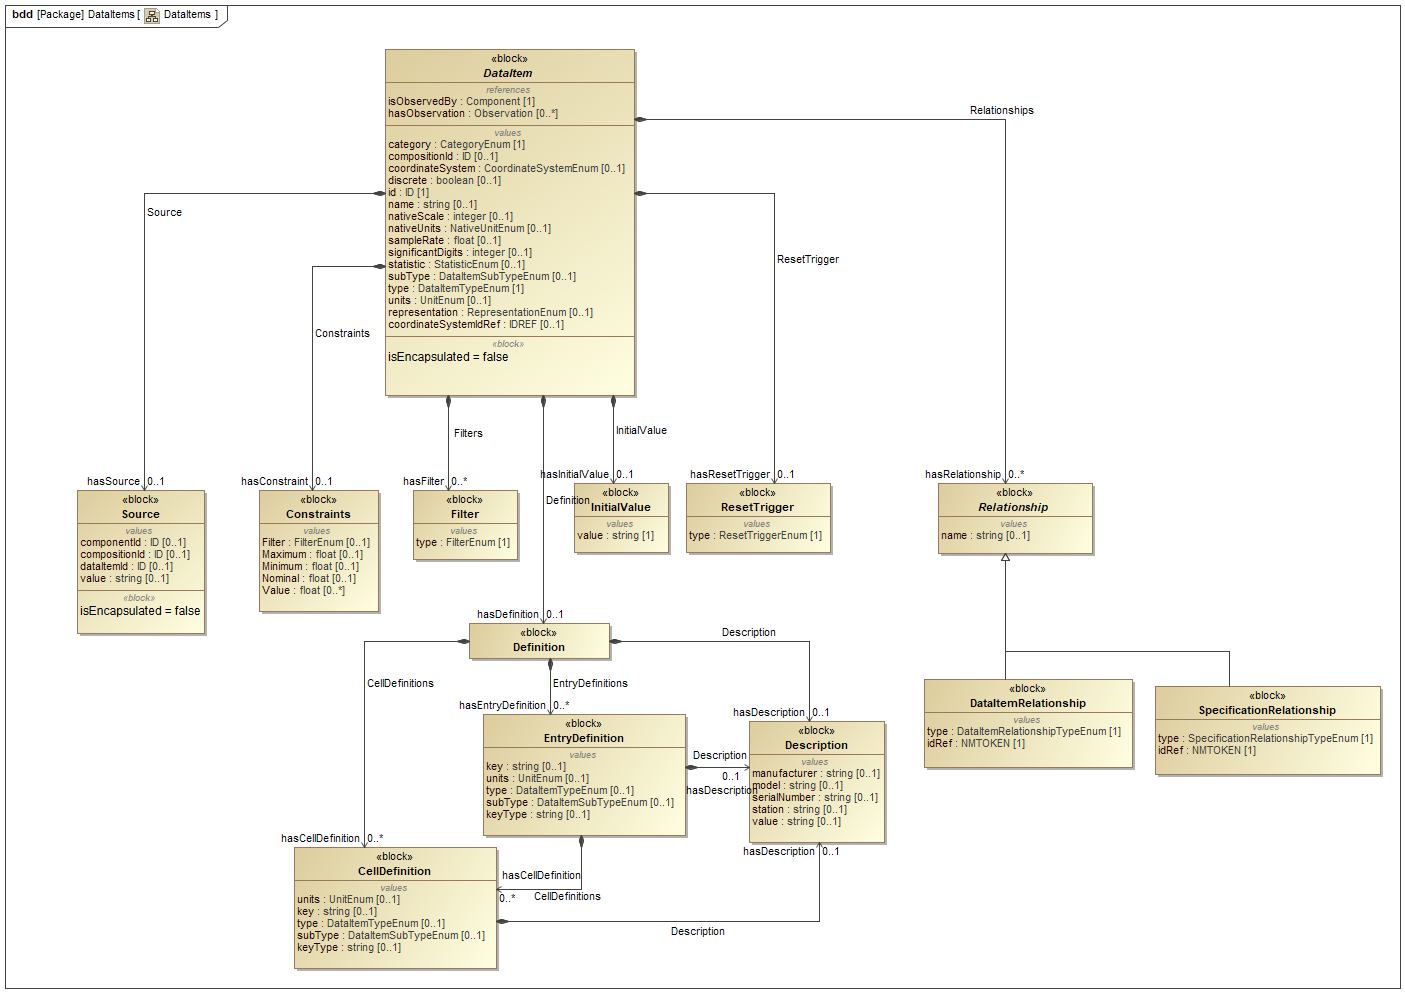
\includegraphics[width=1.0\textwidth]{figures/DataItems.png}
  \caption{DataItems Diagram}
  \label{fig:DataItems}
\end{figure}

\FloatBarrier



\subsubsection{DataItem}
\label{sec:DataItem}



\block{DataItem} describes a piece of information reported about a piece of equipment.


\paragraph{Attributes of DataItem}\mbox{}
\label{sec:Attributes of DataItem}

\tbl{Attributes of DataItem} lists the attributes of \texttt{DataItem}.

\begin{table}[ht]
\centering 
  \caption{Attributes of DataItem}
  \label{table:Attributes of DataItem}
\tabulinesep=3pt
\begin{tabu} to 6in {|l|l|l|} \everyrow{\hline}
\hline
\rowfont\bfseries {Attribute} & {Type} & {Multiplicity} \\
\tabucline[1.5pt]{}
\property{category}[DataItem] & \texttt{CategoryEnum} & 1 \\
\property{compositionId}[DataItem] & \texttt{ID} & 0..1 \\
\property{coordinateSystem}[DataItem] & \texttt{CoordinateSystemEnum} & 0..1 \\
\property{discrete}[DataItem] & \texttt{boolean} & 0..1 \\
\property{id}[DataItem] & \texttt{ID} & 1 \\
\property{name}[DataItem] & \texttt{string} & 0..1 \\
\property{nativeScale}[DataItem] & \texttt{integer} & 0..1 \\
\property{nativeUnits}[DataItem] & \texttt{NativeUnitEnum} & 0..1 \\
\property{sampleRate}[DataItem] & \texttt{float} & 0..1 \\
\property{significantDigits}[DataItem] & \texttt{integer} & 0..1 \\
\property{statistic}[DataItem] & \texttt{StatisticEnum} & 0..1 \\
\property{subType}[DataItem] & \texttt{DataItemSubTypeEnum} & 0..1 \\
\property{type}[DataItem] & \texttt{DataItemTypeEnum} & 1 \\
\property{units}[DataItem] & \texttt{UnitEnum} & 0..1 \\
\property{representation}[DataItem] & \texttt{RepresentationEnum} & 0..1 \\
\property{coordinateSystemIdRef}[DataItem] & \texttt{IDREF} & 0..1 \\
\end{tabu}
\end{table}
\FloatBarrier


Descriptions for attributes of \block{DataItem}:

\begin{itemize}

\item \property{category}[DataItem] : Specifies the kind of information provided by a data item.

\tabulinesep = 5pt
\begin{longtabu} to \textwidth {
    |l|X|}
\caption{CategoryEnum Enumeration}
\label{enum:CategoryEnum} \\

\hline
Name & Description \\
\hline
\endfirsthead
\hline
\multicolumn{2}{|c|}{Continuation of Table \texttt{CategoryEnum} Enumeration} \\
\hline
Name & Description \\
\hline
\endhead
\texttt{SAMPLE} & A \texttt{SAMPLE} is the reading of the value of a continuously variable or analog data value. A continuous value can be measured at any point-in-time and will always produce a result. \\ \hline
\texttt{EVENT} & An \texttt{EVENT} is a data item representing a discrete piece of information from the piece of equipment. \\ \hline
\texttt{CONDITION} & A \texttt{CONDITION} is a data item that communicates information about the health of a piece of equipment and its ability to function. \\ \hline
\end{longtabu}


\item \property{compositionId}[DataItem] : The identifier attribute of the \block{Composition} element that the reported data is most closely associated.

\item \property{coordinateSystem}[DataItem] : For measured values relative to a coordinate system like \block{POSITION}, the coordinate system being used may be reported.

\tabulinesep = 5pt
\begin{longtabu} to \textwidth {
    |l|X|}
\caption{CoordinateSystemEnum Enumeration}
\label{enum:CoordinateSystemEnum} \\

\hline
Name & Description \\
\hline
\endfirsthead
\hline
\multicolumn{2}{|c|}{Continuation of Table \texttt{CoordinateSystemEnum} Enumeration} \\
\hline
Name & Description \\
\hline
\endhead
\texttt{MACHINE} & An unchangeable coordinate system that has machine zero as its origin. \\ \hline
\texttt{WORK} & The coordinate system that represents the working area for a particular workpiece whose origin is shifted within the \texttt{MACHINE} coordinate system. If the \texttt{WORK} coordinates are not currently defined in the piece of equipment, the \texttt{MACHINE}
coordinates will be used. \\ \hline
\end{longtabu}


\item \property{discrete}[DataItem] : An indication signifying whether each value reported for the \gls{Data Entity} is significant and whether duplicate values are to be suppressed.

If a value is not defined for \property{discrete}, the default value \textbf{MUST} be \texttt{false}.

\item \property{id}[DataItem] : The unique identifier for this element.

\item \property{name}[DataItem] : The name of an element or a piece of equipment.

\item \property{nativeScale}[DataItem] : \block{nativeScale} \textbf{MAY} be used to convert the reported value to represent the original measured value.

\item \property{nativeUnits}[DataItem] : The native units of measurement for the reported value of the data item.

\tabulinesep = 5pt
\begin{longtabu} to \textwidth {
    |l|X|}
\caption{NativeUnitEnum Enumeration}
\label{enum:NativeUnitEnum} \\

\hline
Name & Description \\
\hline
\endfirsthead
\hline
\multicolumn{2}{|c|}{Continuation of Table \texttt{NativeUnitEnum} Enumeration} \\
\hline
Name & Description \\
\hline
\endhead
\texttt{CENTIPOISE} & A measure of viscosity. \\ \hline
\texttt{DEGREE/MINUTE} & Rotational velocity in degrees per minute. \\ \hline
\texttt{FAHRENHEIT} & Temperature in Fahrenheit. \\ \hline
\texttt{FOOT} & Feet. \\ \hline
\texttt{FOOT/MINUTE} & Feet per minute. \\ \hline
\texttt{FOOT/SECOND} & Feet per second. \\ \hline
\texttt{FOOT/SECOND\^{}2} & Acceleration in feet per second squared. \\ \hline
\texttt{FOOT\textunderscore 3D} & A point in space identified by X, Y, and Z positions and represented by a space-delimited set of numbers each expressed in feet. \\ \hline
\texttt{GALLON/MINUTE} & Gallons per minute. \\ \hline
\texttt{HOUR} & A measurement of time in hours. \\ \hline
\texttt{INCH} & Inches. \\ \hline
\texttt{INCH/MINUTE} & Inches per minute. \\ \hline
\texttt{INCH/SECOND} & Inches per second. \\ \hline
\texttt{INCH/SECOND\^{}2} & Acceleration in inches per second squared. \\ \hline
\texttt{INCH\textunderscore POUND} & A measure of torque in inch pounds. \\ \hline
\texttt{INCH\textunderscore 3D} & A point in space identified by X, Y, and Z positions and represented by a space-delimited set of numbers each expressed in inches. \\ \hline
\texttt{KELVIN} & A measurement of temperature. \\ \hline
\texttt{KILOWATT} & A measurement in kilowatt. \\ \hline
\texttt{KILOWATT\textunderscore HOUR} & Kilowatt hours which is 3.6 mega joules. \\ \hline
\texttt{LITER} & Measurement of volume of a fluid. \\ \hline
\texttt{LITER/MINUTE} & Measurement of rate of flow of a fluid. \\ \hline
\texttt{MILLIMETER/MINUTE} & Velocity in millimeters per minute. \\ \hline
\texttt{MINUTE} & A measurement of time in minutes. \\ \hline
\texttt{OTHER} & Unsupported units. \\ \hline
\texttt{POUND} & US pounds. \\ \hline
\texttt{POUND/INCH\^{}2} & Pressure in pounds per square inch (PSI). \\ \hline
\texttt{RADIAN} & Angle in radians. \\ \hline
\texttt{RADIAN/MINUTE} & Velocity in radians per minute. \\ \hline
\texttt{RADIAN/SECOND} & Rotational acceleration in radian per second squared. \\ \hline
\texttt{RADIAN/SECOND\^{}2} & Rotational acceleration in radian per second squared. \\ \hline
\texttt{REVOLUTION/SECOND} & Rotational velocity in revolution per second. \\ \hline
\end{longtabu}


\item \property{sampleRate}[DataItem] : The rate at which successive samples of a data item are recorded by a piece of equipment.

\item \property{significantDigits}[DataItem] : The number of significant digits in the reported value.

\item \property{statistic}[DataItem] : Describes the type of statistical calculation performed on a series of data samples to provide the reported data value.

\tabulinesep = 5pt
\begin{longtabu} to \textwidth {
    |l|X|}
\caption{StatisticEnum Enumeration}
\label{enum:StatisticEnum} \\

\hline
Name & Description \\
\hline
\endfirsthead
\hline
\multicolumn{2}{|c|}{Continuation of Table \texttt{StatisticEnum} Enumeration} \\
\hline
Name & Description \\
\hline
\endhead
\texttt{AVERAGE} & Mathematical Average value calculated for the data item during the calculation period. \\ \hline
\texttt{KURTOSIS} & \textbf{DEPRECATED} in \textit{Version 1.6}. \sout{A measure of the "peakedness" of a probability distribution; i.e., the shape of the distribution curve.} \\ \hline
\texttt{MAXIMUM} & Maximum or peak value recorded for the data item during the calculation period. \\ \hline
\texttt{MEDIAN} & The middle number of a series of numbers. \\ \hline
\texttt{MINIMUM} & Minimum value recorded for the data item during the calculation period. \\ \hline
\texttt{MODE} & The number in a series of numbers that occurs most often. \\ \hline
\texttt{RANGE} & Difference between the maximum and minimum value of a data item during the calculation period. Also represents Peak-to-Peak measurement in a waveform. \\ \hline
\texttt{ROOT\textunderscore MEAN\textunderscore SQUARE} & Mathematical Root Mean Square (RMS) value calculated for the data item during the calculation period. \\ \hline
\texttt{STANDARD\textunderscore DEVIATION} & Statistical Standard Deviation value calculated for the data item during the calculation period. \\ \hline
\end{longtabu}


\item \property{subType}[DataItem] : A sub-categorization of the data item \block{type}.

\item \property{type}[DataItem] : The type of either a \gls{Structural Element} or a \block{DataItem} being measured.

\item \property{units}[DataItem] : The unit of measurement for the reported value of the data item.

\tabulinesep = 5pt
\begin{longtabu} to \textwidth {
    |l|X|}
\caption{UnitEnum Enumeration}
\label{enum:UnitEnum} \\

\hline
Name & Description \\
\hline
\endfirsthead
\hline
\multicolumn{2}{|c|}{Continuation of Table \texttt{UnitEnum} Enumeration} \\
\hline
Name & Description \\
\hline
\endhead
\texttt{AMPERE} & Amps \\ \hline
\texttt{CELSIUS} & Degrees Celsius \\ \hline
\texttt{COUNT} & A count of something. \\ \hline
\texttt{DECIBEL} & Sound Level \\ \hline
\texttt{DEGREE} & Angle in degrees \\ \hline
\texttt{DEGREE\textunderscore 3D} & A space-delimited, floating-point representation of the angular rotation in degrees around the X, Y, and Z axes relative to a cartesian coordinate system respectively in order as A, B, and C. If any of the rotations is not known, it \textbf{MUST} be zero (0). \\ \hline
\texttt{DEGREE/SECOND} & Angular degrees per second \\ \hline
\texttt{DEGREE/SECOND\^{}2} & Angular acceleration in degrees per second squared \\ \hline
\texttt{HERTZ} & Frequency measured in cycles per second \\ \hline
\texttt{JOULE} & A measurement of energy. \\ \hline
\texttt{KILOGRAM} & Kilograms \\ \hline
\texttt{LITER} & Measurement of volume of a fluid \\ \hline
\texttt{LITER/SECOND} & Liters per second \\ \hline
\texttt{MICRO\textunderscore RADIAN} & Measurement of Tilt \\ \hline
\texttt{MILLIMETER} & Millimeters \\ \hline
\texttt{MILLIMETER\textunderscore 3D} & A point in space identified by X, Y, and Z positions and represented by a space-delimited set of numbers each expressed in millimeters. \\ \hline
\texttt{MILLIMETER/REVOLUTION} & Millimeters per revolution. \\ \hline
\texttt{MILLIMETER/SECOND} & Millimeters per second \\ \hline
\texttt{MILLIMETER/SECOND\^{}2} & Acceleration in millimeters per second squared \\ \hline
\texttt{NEWTON} & Force in Newtons \\ \hline
\texttt{NEWTON\textunderscore METER} & Torque, a unit for force times distance. \\ \hline
\texttt{OHM} & Measure of Electrical Resistance \\ \hline
\texttt{PASCAL} & Pressure in Newtons per square meter \\ \hline
\texttt{PASCAL\textunderscore SECOND} & Measurement of Viscosity \\ \hline
\texttt{PERCENT} & Percentage \\ \hline
\texttt{PH} & A measure of the acidity or alkalinity of a solution. \\ \hline
\texttt{REVOLUTION/MINUTE} & Revolutions per minute \\ \hline
\texttt{SECOND} & A measurement of time. \\ \hline
\texttt{SIEMENS/METER} & A measurement of Electrical Conductivity \\ \hline
\texttt{VOLT} & Volts \\ \hline
\texttt{VOLT\textunderscore AMPERE} & The measurement of the apparent power in an electrical circuit, equal to the product of root-mean-square (RMS) voltage and RMS current (commonly referred to as VA). \\ \hline
\texttt{VOLT\textunderscore AMPERE\textunderscore REACTIVE} & The measurement of reactive power in an AC electrical circuit (commonly referred to as VAR). \\ \hline
\texttt{WATT} & Watts \\ \hline
\texttt{WATT\textunderscore SECOND} & Measurement of electrical energy, equal to one Joule \\ \hline
\texttt{REVOLUTION/SECOND} & Revolutions per second. \\ \hline
\texttt{REVOLUTION/SECOND\^{}2} & Revolutions per second squared. \\ \hline
\texttt{GRAM/CUBIC\textunderscore METER} & Gram per cubic meter. \\ \hline
\texttt{CUBIC\textunderscore MILLIMETER} & Geometric volume in millimeters. \\ \hline
\texttt{CUBIC\textunderscore MILLIMETER/SECOND} & Change of geometric volume per second. \\ \hline
\texttt{CUBIC\textunderscore MILLIMETER/SECOND\^{}2} & Change in geometric volume per second squared. \\ \hline
\texttt{MILLIGRAM} & Milligram. \\ \hline
\texttt{MILLIGRAM/CUBIC\textunderscore MILLIMETER} & Milligram per cubic millimeter. \\ \hline
\texttt{MILLILITER} & Milliliter. \\ \hline
\end{longtabu}


\item \property{representation}[DataItem] : Description of a means to interpret data consisting of multiple data points or samples reported as a single value.  

If \property{representation} is not specified, it \textbf{MUST} be determined to be \texttt{VALUE}.


\tabulinesep = 5pt
\begin{longtabu} to \textwidth {
    |l|X|}
\caption{RepresentationEnum Enumeration}
\label{enum:RepresentationEnum} \\

\hline
Name & Description \\
\hline
\endfirsthead
\hline
\multicolumn{2}{|c|}{Continuation of Table \texttt{RepresentationEnum} Enumeration} \\
\hline
Name & Description \\
\hline
\endhead
\texttt{TIME\textunderscore SERIES} & A series of sampled data.

The data is reported for a specified number of samples and each sample is reported with a fixed period. \\ \hline
\texttt{VALUE} & The measured value of the sample data.

If no \property{representation}[DataItem] is specified for a data item, the \property{representation}[DataItem] \textbf{MUST} be determined to be \texttt{VALUE}. \\ \hline
\texttt{DATA\textunderscore SET} & The reported value(s) are represented as a set of \glspl{key-value pair}.

Each reported value in the \gls{Data Set} \textbf{MUST} have a unique key. \\ \hline
\texttt{DISCRETE} & \textbf{DEPRECATED} as a \property{representation} in \textit{MTConnect Version. 1.5}. Replaced by the \property{discrete}[DataItem] attribute of a \block{DataItem}. \\ \hline
\texttt{TABLE} & A \gls{Table} is a two dimensional set of \glspl{key-value pair} where the \block{Entry} represents a row, and the value is a set of \gls{key-value pair} \block{Cell} elements. The \gls{Table} follows the same behavior as the \gls{Data Set} for change tracking, clearing, and history. When an \block{Entry} changes, all \block{Cell} elements update as a single unit following the behavior of a \gls{Data Set}.

Note 1 to Entry: It is best to use the \block{Variable} \block{DataItem} \property{type} if the \block{Cell} elements represent multiple
semantic types.

Each \block{Entry} in the \gls{Table} \textbf{MUST} have a unique key. Each \block{Cell} of each \block{Entry} in the \gls{Table} \textbf{MUST} have a unique key.

See \textit{Section 5.6.5} of \citetitle{MTCPart3}, for a description of
\block{Entry} and \block{Cell} elements. \\ \hline
\end{longtabu}


\item \property{coordinateSystemIdRef}[DataItem] : The associated \block{CoordinateSystem} context for the \block{DataItem}.
\end{itemize}

\paragraph{Elements of DataItem}\mbox{}
\label{sec:Elements of DataItem}

\tbl{Elements of DataItem} lists the elements of \texttt{DataItem}.

\begin{table}[ht]
\centering 
  \caption{Elements of DataItem}
  \label{table:Elements of DataItem}
\tabulinesep=3pt
\begin{tabu} to 6in {|l|l|l|} \everyrow{\hline}
\hline
\rowfont\bfseries {Element Name} & {Type} & {Multiplicity} \\
\tabucline[1.5pt]{}
\block{Source} & \texttt{Source} & 0..1 \\
\block{Constraints} & \texttt{Constraints} & 0..1 \\
\block{Filters} & \texttt{Filter} & 0..* \\
\block{InitialValue} & \texttt{InitialValue} & 0..1 \\
\block{ResetTrigger} & \texttt{ResetTrigger} & 0..1 \\
\block{Definition} & \texttt{Definition} & 0..1 \\
\end{tabu}
\end{table}
\FloatBarrier


Descriptions for elements of \block{DataItem}:

\begin{itemize}
\item \block{Source} : \block{Source} identifies the \block{Component}, \block{DataItem}, or \block{Composition} representing the area of the piece of equipment from which a measured value originates.
\item \block{Constraints} : \block{Constraints} \glspl{organize} a set of expected values that can be reported for this \block{DataItem}.
\item \block{Filters} : \block{Filters} \glspl{organize} the \block{Filter} elements associated with this \block{DataItem} element. 
\item \block{InitialValue} : \block{InitialValue} defines the starting value for a data item as well as the value to be set for the data item after a reset event.
\item \block{ResetTrigger} : \block{ResetTrigger} identifies the type of event that may cause a reset to occur.
\item \block{Definition} : The \block{Definition} defines the meaning of \block{Entry} and \block{Cell} elements associated with the \block{DataItem} when the \property{representation} is either \block{DATA} or \block{TABLE}.
\end{itemize}
